\chapter{Reconstrucción e identificación de objetos físicos}
\label{cap:objetos}


Los objetos fisicos resultantes de las particulas originadas en las colisiones
$pp$ son reconstruidos a partir de las senales provenientes del detector ATLAS.
La reconstruccion de estos objetos no se realiza en tiempo real mientras se
colectan datos (\emph{online}), sino que se realiza luego de que la toma de
datos fue realizada (\emph{offline}).

En este capítulo se describe la reconstrucción, calibración e identificación de
los principales objetos físicos utilizados en el presente análisis: fotones,
jets, muones, electrones y energía faltante. Notar que la correcta
identificación de todos los objetos en el evento es requerida para que el
cálculo de la energía faltante, que es la energía de las partículas que escapan
el detector, sea lo mas preciso posible.


\section{Reconstruccion de trazas y vertices}
\label{sec:obj_vertex}

\hl{Agregar}

%% La reconstruccion del vertice primaro consta de dos pasos []. Primero se realiza
%% la busqueda de los vertices
%% reconstruye una coleccion de vertices a partir de las trazas reconstruidas en el
%% detector interno, preseleccionadas a find de remover aquellas producidas en
%% interacciones secundarias. La posicion del vertice es determinada mediante un
%% algoritmo de ajuste $\chi^2$ sobre el vertice y las trazas de su entorno. Entre
%% todos los candidatos hallados, se elige como primario aquel vertice que maximiza
%% $\sum_{\text{trazas}} \pt^2$.



\section{Fotones y electrones}
\label{sec:obj_photons}

La reconstrucción de fotones y electrones en ATLAS se basa en las deposiciones
locales de energía halladas en el calorímetro electromagnético. Como fotones y
electrones dejan señales similares en el calorímetro electromagnético, su
reconstrucción se realiza en paralelo. La distinción entre unos y otros se
realiza mediante la información de las trazas reconstruidas en el detector
interno.

A fin de reducir la gran contaminación de falsos candidatos a fotones en la
muestra reconstruida debido, principalmente, al decaimiento de mesones livianos,
como por ejemplo $\pi^0 \to \gam\gam$, se aplica una serie de criterios de
identificación, basados en las características de las lluvias electromagnéticas
esperadas en cada caso, y tambien criterios de aislamiento.


\subsection{Reconstrucción}

La lógica de reconstrucción se basa en un algoritmo de clusterización que busca
deposiciones locales de energía en el calorímetro electromagnético dentro de una
ventana rectangular en el plano $(\eta, \phi)$ de tamaño fijo (\emph{sliding
  window algorithm}) \cite{Delmastro:1747242}. La posición de la ventana se
ajusta buscando que la energía transversa de todas las celdas contenidas sea un
máximo local, con un mínimo de 2.5 \gev. El tamaño óptimo de la ventana depende
del tipo de partícula a reconstruir y de la región del calorímetro. Las lluvias
electromagnéticas iniciadas por electrones son en general mas anchas que las de
fotones, debido a su mayor probabilidad de interacción con el material previo al
calorímetro electromagnético y a la radiación de fotones de bremsstrahlung. La
energía total y la posición de estos clusters es luego calibrada, separadamente
para electrones y fotones, a fin de tener en cuenta diversos efectos como la
perdida de energía en el material inactivo del calorímetro o la deposición
lateral y longitudinal fuera del cluster. A partir de simulaciones Monte Carlo,
se estima que la eficiencia de esta reconstrucción inicial sea del 100\% para
objetos con $\et > 20 \gev$.

Como punto de partida en la separación de electrones y fotones, las trazas,
reconstruidas en el detector interno, son asociadas a un cluster si la distancia
entre el baricentro del cluster y el punto de intersección de la traza
extrapolada con la segunda capa del calorímetro es menor a 0.05 en $\eta$ y 0.05
(0.2) en $\phi$ en la dirección a (opuesto a) la curvatura de las trazas en el
campo magnético del solenoide de ATLAS. Solo las trazas asociadas de esta forma
con un cluster son retenidas para la reconstrucción de electrones y fotones.

Aquellos clusters electromagnéticos asociados en el espacio $(\eta,\phi)$ con
una traza reconstruida con $\pt > 0.5 \gev$ son clasificados como electrones. La
definición para fotones es un poco mas compleja ya que estos pueden convertir en
un par $e^+e^-$ en el volumen anterior al calorímetro. Los fotones convertidos
están caracterizados por la presencia de al menos una traza asociada proveniente
de un vértice reconstruido en el ID. La probabilidad de conversión varia entre
un 40\% y un 80\%, aunque solo aquellas que ocurren antes del TRT son
eficientemente reconstruidas.

Los fotones son clasificados como \emph{no-convertidos} si no tienen trazas de
un vértice de conversión asociadas al cluster, y como \emph{convertidos} en el
caso contrario. Un vértice de conversión es formado cuando dos trazas que pasan
un cierto umbral en el TRT, forman un vértice consistente como provenientes de
una partícula no masiva. Para aumentar la eficiencia de reconstrucción de
fotones convertidos, los candidatos a conversión donde solo una de las dos
trazas es reconstruida (y no tiene ningún impacto en la capa más interior del
detector de pixeles) también son retenidas.

Un algoritmo final \cite{PhotonPerf} se utiliza para resolver la
ambigüedad entre candidatos a fotones convertidos que son también reconstruidos
como electrones y permite la recuperación de fotones que fueron inicialmente
clasificados como candidatos a electrones.
Para candidatos a fotones convertidos que también son reconstruidos como
electrones, se evalúa la traza del electrón contra la traza originada del
candidato a vértice de conversión asociada al mismo cluster. Si la traza
coincide con una traza proveniente de un vértice de conversión, el candidato a
fotón convertido es retenido.

%% The only exception is the case of a double-track conversion vertex candidate where the coinciding track
%% has a hit in the b-layer, while the other track lacks one (for this purpose, a missing hit in a disabled b-layer
%% module is counted as a hit 2
%% ). If the track does not coincide with any of the tracks assigned to the conver-
%% sion vertex candidate, the converted photon candidate is removed, unless the track pT is smaller than that
%% of the candidate converted photon pT.

Cuando se calcula el {\pt} del fotón, la energía es tomada siempre del cluster
del calorímetro, apropiadamente calibrada\cite{Banfi:1259219}. Para fotones
no-convertidos, el $\eta$ es calculado usando las dos primeras capas del
calorímetro electromagnético. Para fotones convertidos, donde la traza o las
trazas que provienen del vértice de la conversión contiene mas de tres impactos en
el detector de silicio, la dirección $\eta$ se determina extrapolando del
cluster del calorímetro al vértice de la conversión. Para fotones convertidos
que tienen trazas solo en el TRT, $\eta$ es calculada del calorímetro, % calorimeter pointing
como en el caso de los no-convertidos.
%% Además, la escala de energía
%% del fotón es corregida para datos y \hl{smeareada} para las muestras de MC.

De simulaciones Monte Carlo, se calcula que el 96\% de los fotones con
$\et>25\gev$ son reconstruidos como candidatos a fotón, mientras que el 4\%
restante son incorrectamente reconstruidos como electrones. % de ATL-COM-PHYS-2014-949

En el caso de electrones, la eficiencia de reconstrucción es de alrededor de
97\% para electrones con $\et=15 \gev$ y alcanza $99 \%$ para $\et=50\gev$. Esta
eficiencia varia de 99\% a bajo $|\eta|$ hasta 95\% a alto $|\eta|$ (para
electrones con $\et>15 \gev$). %% de ATLAS-CONF-2014-032


\subsection{Identificación de fotones}
\label{sec:fotones}

Para distinguir entre candidatos a ser fotones reales de fotones de fondo, es
necesario contar con un algoritmo de identificación con una alta eficiencia y un alto rechazo
de fondo, para candidatos con {\et} desde los 10 {\gev} hasta la escala del
{\tev}. La identificación de fotones se basa en un conjunto de cortes
rectangulares en una serie de variables discriminatorias que (se detallan a continuación)
que caracterizan el desarrollo lateral y longitudinal de la
lluvia en el calorímetro electromagnético y la fracción de la lluvia filtrada en
el calorímetro hadrónico. Los fotones reales producen generalmente depósitos de
energía mas angostos en el calorímetro electromagnético y tienen una menor
filtración en el calorímetro hadrónico, comparado con los fotones de fondo
provenientes generalmente de jets, debido a la presencia de hadrones adicionales cercanos al
candidato a fotón. Además, los candidatos provenientes de
decaimientos aislados $\pi^0 \to \gam\gam$, están caracterizados por dos máximos
locales de energía separados, en las \emph{strips} de la primer capa del calorímetro,
debido a la presencia de los dos fotones cercanos.

A continuación se detallan las variables discriminatorias utilizadas en la identificación de fotones. La primera
 variable utiliza la energía medida en el calorímetro hadrónico:

\begin{itemize}\itemsep0.2cm\parskip0.2cm

\item Filtración hadrónica: es la energía transversa depositada en el
  calorímetro hadrónico, normalizada a la energía transversa del cluster
  electromagnético

  \begin{equation}
    R_{\mathrm{had}_{(1)}} = \frac{\et^{\mathrm{had}}}{\et}
  \end{equation}

  En la región de transición barrel-endcap del HCAL ($0.8\leq |\eta| \leq 1.37$) se utiliza
  el deposito de energía en todo el calorímetro hadrónico para minimizar los efectos de la
  degradación de resolución ($R_{\mathrm{had}}$). En el resto del detector, se mide solo la
  energía hadrónica depositada en la primera capa del HCAL ($R_{\mathrm{had}_{(1)}}$).
\end{itemize}

Las siguientes variables utilizan la información de la segunda capa del calorímetro electromagnético:

\begin{itemize}\itemsep0.2cm\parskip0.2cm
\item Perfil lateral de energía en $\eta$

  \begin{equation}
    R_\eta = \frac{E^{s2}_{3\times 7}}{E^{s2}_{7\times 7}}
  \end{equation}
%
  donde $E^{s2}_{i\times j}$ es la suma de las celdas en la segunda capa del calorímetro
  electromagnético contenidas en una ventana $i \times j$ (en unidades de celda $\eta \times \phi$).

\item Perfil lateral de energía en $\phi$

  \begin{equation}
    R_\phi = \frac{E^{s2}_{3\times 3}}{E^{s2}_{3\times 7}}
  \end{equation}

  definida en modo similar a $R_\eta$.
  $R_\phi$, sin embargo, se comporta muy distinto para fotones convertidos y
  fotones no convertidos. Por acción del campo magnético, los electrones y positrones
  generados en la conversión curvan su trayectoria en direcciones opuestas en $\phi$,
  dando lluvias electromagnéticas mas anchas que los fotones no convertidos en esta dirección
  como se esquematiza en la fig.


  \item RMS del perfil lateral de energía en $\eta$

  \begin{equation}
    w_{\eta_2} = \sqrt{ \frac{\sum E_i \eta_i^2}{\sum E_i} - \left( \frac{\sum E_i \eta_i}{\sum E_i} \right) }
  \end{equation}
  %
  mide el ancho lateral de las lluvias electromagnéticas, donde $E_i$ es la energía de la i-esima celda del
  calorímetro electromagnético contenida en una ventana $3 \times 5$ celdas en $\eta \times \phi$.
\end{itemize}

Las siguientes son las variables que utilizan la información de la primera capa
del calorímetro electromagnético, la cual esta compuesta por celdas en forma de
bandas (strips) que permiten una muy buena separación entre fotones aislados y
fotones provenientes del decaimimietno del $\pi^0$. La \hl{Fig} muestra el perfil de
una lluvia electromagnética típica de cada tipo en eventos de datos reales donde
se puede apreciar la estructura del perfil de energía en la primera capa del
ECAL en el caso de un decamiento $\pi^0 \to \gam\gam$.

\begin{itemize}\itemsep0.2cm\parskip0.2cm
\item Perfil lateral de energía en $\eta$

  \begin{equation}
    F_\mathrm{side} = \frac{E(\pm 3) - E(\pm 1)}{E(\pm 1)}
  \end{equation}
  %
  mide la contención lateral de la cascada electromagnética a lo largo de $\eta$.
  $E(\pm n)$ es la energía en las $\pm n$ celdas alrededor de aquella con la deposición máxima.

\item RMS del perfil lateral de energía en $\eta$ (3 strips)

  \begin{equation}
    w_{s,3} = \sqrt{ \frac{\sum E_i (i - i_\mathrm{max})^2}{\sum E_i} }
  \end{equation}
  %
  mide el ancho de la lluvia electromagnética a lo largo de $\eta$ en la primera capa
  del calorímetro electromagnético usando solo la banda con mayor deposición de energía ($E_{i_\mathrm{max}}$)
  y sus vecina inmediatas.

\item RMS del perfil lateral de energia en eta (total)

  $w_{s,\mathrm{tot}}$ esta definida de la misma forma que $w_{s,3}$, pero utiliza todas las bandas de la
  primera capa del calorimetro electromagnética en una ventana $\Delta\eta \times \Delta\phi = 0.0625 \times 0.2$,
  que corresponde aproximadamente a $20 \times 2$ bandas en $\eta \times \phi$.

\item Diferencia al segundo maximo

  \begin{equation}
    \Delta E = (E^{s1}_{2^{\mathrm{do}} max} - E_\mathrm{min}^{s1} )
  \end{equation}
  %
  es la diferencia entre la energía de la banda con la segunda energía más grande ($E^{s1}_{2^{\mathrm{do}} max}$),
  y la mínima energía ($E_\mathrm{min}^{s1}$) entre la anterior y la celda con la máxima deposición. En caso
  de no haber segundo máximo se fija $\Delta E = 0$.

\item Asimetría de los dos máximos locales en $\eta$

  \begin{equation}
    E_\mathrm{ratio} = \frac{ E^{s1}_{1^{\mathrm{st}} max} - E^{s1}_{2^{\mathrm{nd}} max} }{ E^{s1}_{1^{\mathrm{st}} max} + E^{s1}_{2^{\mathrm{nd}} max} }
  \end{equation}
  %
  mide la diferencia relativa entre las energías de las dos celdas con máxima deposición. En caso de no haber segundo máximo
  se fija $E_\mathrm{ratio} = 1$.

\end{itemize}


A partir de estas variables discriminatorias se definen dos conjuntos de cortes: \emph{loose} y
\emph{tight}.
La selección \emph{loose} se basa solo en las formas de la lluvia
en la segunda capa del calorímetro EM y en la energía depositada en el
calorímetro hadrónico, y es utilizada especialmente por el trigger. La selección
\emph{tight} agrega además información de la capa de \emph{strips} del calorímetro, que
provee un buen rechazo de fondo, %jets hadronicos en los cuales el mesón neutro lleva la mayor parte de la energía del jet
además de ajustar los cortes en las
demás variables. Las variables utilizadas en cada conjunto pueden verse detalladas
en la \cref{tab:phel_id}.

Los cortes de cada conjunto de identificación en las variables que
describen la forma de la lluvia son independientes de la energía transversa del
candidato a fotón, pero varían según la pseudo-rapidez reconstruida del fotón,
para tener en cuenta las variaciones en la cantidad de material y la geometría
del calorímetro.
La selección \emph{tight} se optimiza de forma separada para
fotones convertidos y no-convertidos para proveer una eficiencia de
identificación de alrededor de 85\% para candidatos a fotón con energía
transversa $\et>40 \gev$ y un alto rechazo de fondo\cite{PhotonPerf}.

%% En áreas donde un modulo de la b-layer esta muerto, los electrones son
%% comúnmente reconstruido como fotones convertidos. Esta ambigüedad es resulta
%% teneinedo en cuenta el mapa de los píxeles muertos como función del tiempo que
%% dura la recolección de datos. Las conversiones con una sola traza falsas (y
%% algunas de dos trazas) son de esta forma reducidas, con solo un mínima reducción
%% de la eficiencia.


\begin{table}[!htbp]

  \centering

  \caption{Definición de las diferentes variables usadas para la selección
    \emph{loose} (L), \emph{medium} (M) y \emph{tight} (T) de fotones y
    electrones. Las cruces ``x'' indican las variables que son utilizadas en
    cada selección. Además de las variables adicionales utilizadas en cada
    caso, también se incrementan los cortes en las mismas.}
  \label{tab:phel_id}

  \begin{tabular}{l p{7cm} c | cc | ccc}

    \hline
    &            &                                       & \multicolumn{2}{c}{$\gamma$} & \multicolumn{3}{c}{$e$} \\
    Categoria    & Descripción                                      & Nombre                  & L & T & L & M & T \\
    \hline

  Aceptancia     & $|\eta|<2.37$, excluyendo $1.37<|\eta|<1.52$       & -                       &   & $\times$ &   & $\times$ & $\times$ \\


  Fuga hadrónica & Cociente entre {\et} en la primera capa del
                   calorímetro hadrónico y {\et} del
                   cluster electromagnético
                   ($|\eta|<0.8$ y $|\eta|\geq1.37$)                & $R_{\mathrm{had}_1}$    & $\times$ & $\times$ & $\times$ & $\times$ & $\times$ \\

                 & Cociente entre {\et} en todo el calorímetro
                   hadrónico y {\et} del cluster electromagnético
                   ($|\eta|\leq0.8$ y $|\eta|<1.37$)                & $R_{\mathrm{had}}$      & $\times$ & $\times$ & $\times$ & $\times$ & $\times$ \\


  EM ($2^\mathrm{da}$ capa)  & Cociente entre la suma de las energías de las
                   $3\times7$ celdas y la suma de $5\times 7$
                   celdas, ambas en torno al centro del cluster     & $R_\eta$                & $\times$ & $\times$ & $\times$ & $\times$ & $\times$ \\

                 & Ancho lateral de la lluvia en dirección de
                   $\eta$                                           & $w_{\eta_2}$            & $\times$ & $\times$ & $\times$ & $\times$ & $\times$ \\

                 & Cociente entre la suma de las energías de las
                   $3\times 3$ celdas y la suma de $3\times 7$
                   celdas, ambas en torno al centro del cluster     & $R_\phi$                &   & $\times$ & $\times$ & $\times$ & $\times$ \\


  EM ($1^\mathrm{ra}$ capa) & Ancho lateral de la lluvia en 3 strips alrededor
                  del máximo                                        & $w_{s,3}$               &   & $\times$ &   & $\times$ & $\times$ \\

                & Ancho lateral total de la lluvia                  & $w_{s,\mathrm{tot}}$    &   & $\times$ &   & $\times$ & $\times$ \\

                & Fracción de energía fuera de las 3 strips
                  centrales pero dentro de las 7                    & $F_{\mathrm{side}}$     &   & $\times$ &   & $\times$ & $\times$ \\

                & Diferencia entre la energía de la strip con el
                  segundo mayor depósito y la menor energía entre
                  los dos primeros máximos locales                  & $\Delta E$              &   & $\times$ &   & $\times$ & $\times$ \\

                & Asimetría entre el primer y segundo máximo        & $E_{\mathrm{ratio}}$    &   & $\times$ &   & $\times$ & $\times$ \\


  ID            & Impactos en el Pixel $\geq 1$ y en el
                  SCT $\geq 7$                                      & -                       &   &   &   & $\times$ & $\times$ \\

                & Parámetro de impacto $\leq \unit[1]{mm}$          & -                       &   &   &   & $\times$ & $\times$ \\


  EM+ID         & $\Delta\eta,\Delta\phi$ entre la traza
                  extrapolada al calorímetro y el cluster           & $\Delta\eta,\Delta\phi$ &  &   &   & $\times$ & $\times$ \\

                & Cociente entre la energía del cluster y el impulso
                  de la traza                                       & $E/p$                   &  &   &   & $\times$ & $\times$ \\


  TRT           & Impactos en el TRT                                & -                       &  &   &   & $\times$ & $\times$ \\

                & Fracción de impactos de alto umbral en el TRT     & -                       &  &   &   & $\times$ & $\times$ \\
  \hline
  \end{tabular}

\end{table}



\subsubsection{Corrección a las variables de identificación}

%% Significant differences are observed between data and MC in the shower shape
%% (isEM) distributions.

Dado que la simulación del detector no es perfecta, las distribuciones de las variables
discriminatorias utilizadas en la identificación
de fotones presentan algunas diferencias que pueden resultar significativas entre datos y MC.
Estas diferencias pueden parametrizarse a primer orden como variaciones simples
y a partir de estos corregir el MC.
Las diferencias para cada variable discriminatoria (DV$^i$) se calcula
comparando las distribuciones de las mismas en los datos y en una muestra de
Monte Carlo con una mezcla similar de eventos de señal y fondo.
A partir de esto se calcula la diferencia
entre los valores medios, lo que se denomina \emph{fudge-factor} ($\mu^i$)\cite{ATLAS-CONF-2012-123}.

\begin{equation}
  \Delta \mu^i = \avg{\mathrm{DV}^i_\text{DATA}} - \avg{\mathrm{DV}^i_\mathrm{MC}}
\end{equation}

Estos factores son utilizados para corregir las variables de las
muestras simuladas, y los cortes de identificación son nuevamente
aplicados a las variables corregidas.
%% La eficiencia de identificación
%% de fotones es por lo tanto ajustadas para igualar las medidas en datos.

%% Una aproximación mas sofisticada para obtener estas diferencias consiste
%% en minimizar la función $\chi^2$ entre las distribuciones de datos y MC,
%% mejorando considerablemente el acuerdo, y es
%% el metodo que se utiliza en el analisis.

%% A more
%% sophisticated approach obtains the shifts by minimizing a chi2 between the data
%% and MC distributions. This method is imperfect in that a shift does not take
%% into account differences in the shape of the distributions and in that it
%% assumes that the shifts are the same for signal and background. However it has
%% been shown that it improves the agreement with data significantly and it is
%% therefore recommended for 2010, 2011, and 2012 photon analyses. A set of shifts
%% has been tabulated for the 2010, 2011, and 2012 data-sets, independently. The MC
%% sample corrected in this way are referred to here as the FF-MC. For 2010 the
%% uncertainty on the FF-MC PID efficiency prediction was conservatively tabulated
%% without the use of data-driven methods, by comparing the efficiencies obtained
%% using different selection criteria and carrying out closure tests using
%% distorted samples as detailed in ATL-PHYS-INT-2011-014 and
%% ATL-COM-PHYS-2011-645 in page 19, and finally at lower  in
%% ATL-COM-PHYS-2011-301 in page 78. For the later data periods the uncertainty is
%% determined through comparisons to data-driven methods and in 2011 additional
%% ``Scale Factors'' are recommended.

También es necesario aplicar factores de escala a todos los fotones
identificados en las muestras de MC para tener en cuenta las diferencias
observadas en la eficiencia de identificación respecto a los datos. Estos
factores son derivados de forma separada para fotones convertidos y
no-convertidos son provistos de forma central por el grupo
\textsc{Egamma} de ATLAS.


\subsubsection{Aislamiento}

Para la selección final de fotones, se aplica además un corte en la energía
transversa de aislamiento {\etiso}.

%% La energía de aislamiento se define como la
%% suma de la energía transversa de los clusters topologicos (apropiadamente calibrada)
%% dentro de un cono en el plano $(\eta, \phi)$ de radio $R$ alrededor del baricentro del cluster.
%% Solo los topoclusters con energía positiva son usados. Los topoclusters
%% incluyen celdas del calorímetro electromagnético y del calorímetro hadrónico, pero
%% las celdas del TileGap3 son explícitamente removidas.
%% La energía del centro del cono en el calorímetro electromagnético ($5\times7$ celdas alrededor el
%% baricentro del objeto) es sustraída de la suma. Luego se aplican correcciones
%% debido a la energía ambiente por la actividad del pile-up calculadas de acuerdo
%% a \cite{Hance:1379530}, mejorando la performance de la variable de aislamiento
%% para alto pile-up \cite{Laplace:1444890}.


%% Se observa una diferencia entre la energía filtrada del fotón en el cono de
%% aislamiento para datos y MC. Por lo tanto, las correcciones aplicadas que se
%% describen en \cite{Hance:1379530} son levemente distintas para datos y MC.
%% Incluso, se observa que existe una dependencia remanente en la energía de
%% aislamiento con el {\pt} del fotón en datos, para lo cual se aplica un factor de
%% corrección extra que se describe en \cref{sec:opt_ph_iso}.

%% La energia de aislamiento
%% depues de aplicarle las correciones tiene que ser menor que 5 {\gev} para
%% pasar la seleccion final.

%% Los fotones pre-seleccionados son entonces lo que tienen un {\pt} mayor a 20
%% {\gev} con $|\eta| < 2.37$, removiendo los que se encuentran en la región del
%% crack $1.37 < |\eta| < 1.52$, donde $\eta$ se mide en el cluster de la segunda
%% capa del calorímetro.

%% \subsection{Correciones para fotones}

%% Algunas correcciones son aplicadas para mejorar el acuerdo entre datos y
%% simulaciones MC del modelado de las lluvias que dejan los fotones al
%% pasar por el detector.


\begin{figure}[!htbp]
  \centering

  \resizebox{0.5\textwidth}{!}{
    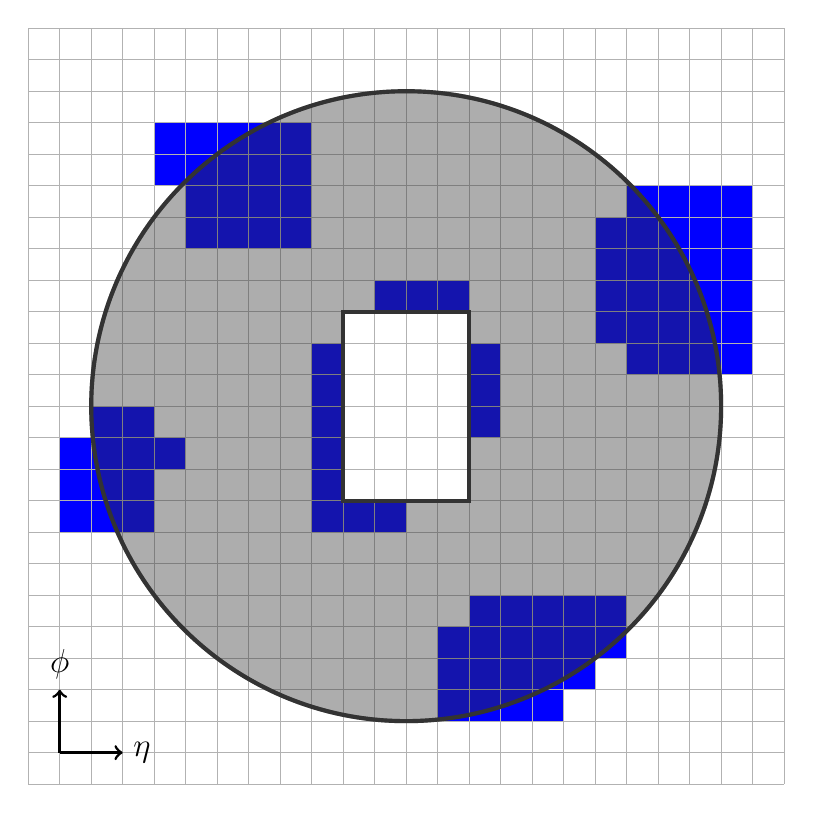
\begin{tikzpicture}

  %% middle
  \draw[blue,fill] (-1.2, -0.4) rectangle (1.2,0.4);
  \draw[blue,fill] (-0.8, -0.8) rectangle (0.8,0.0);
  \draw[blue,fill] (-1.2, 0.4) rectangle (1.2,0.8);
  \draw[blue,fill] (-0.4, -0.8) rectangle (0.4,-1.2);
  \draw[blue,fill] (-0.4, 0.8) rectangle (0.8,1.6);
  \draw[blue,fill] (-1.2, -0.0) rectangle (-0.0,-1.6);

  %% izq arriba
  \draw[blue,fill] (-1.2, 2) rectangle (-2.8,3.6);
  \draw[blue,fill] (-2.8, 3.2) rectangle (-3.2, 3.6);
  \draw[blue,fill] (-2.8, 2.8) rectangle (-3.2, 3.2);

  %% izq abajo
  \draw[blue,fill] (-3.2, -0.4) rectangle (-4.4,-1.6);
  \draw[blue,fill] (-2.8, -0.4) rectangle (-3.2,-0.8);
  \draw[blue,fill] (-3.2, -0.0) rectangle (-4.0,-0.4);

  %% der arriba
  \draw[blue,fill] (2.8, 0.4) rectangle (4.4,2.8);
  \draw[blue,fill] (2.4, 0.8) rectangle (2.8,2.4);

  %% der abajo
  \draw[blue,fill] (0.4, -2.8) rectangle (2.0,-4.0);
  \draw[blue,fill] (0.8, -2.4) rectangle (2.0,-2.8);
  \draw[blue,fill] (2.0, -2.4) rectangle (2.4,-3.6);
  \draw[blue,fill] (2.4, -2.4) rectangle (2.8,-3.2);

  % grid/cone
  \draw[step=0.4,black!30,thin] (-4.8,-4.8) grid (4.8,4.8);

  \draw[black!80, line width=1.5] (0,0) circle (4);
  \draw[black!80, line width=1.5, fill, opacity=0.4] (0,0) circle (4);

  \draw[black!80, line width=1.5, fill=white] (-0.8,-1.2) rectangle (0.8,1.2);
  \draw[step=0.4,black!30,thin] (-0.8,-1.2) grid (0.8,1.2);
  \draw[black!80, line width=1.5] (-0.8,-1.2) rectangle (0.8,1.2);


  \draw[->, line width=1] (-4.4,-4.4) -- (-3.6,-4.4) node[right] {\large $\eta$};
  \draw[->, line width=1] (-4.4,-4.4) -- (-4.4,-3.6) node[above] {\large $\phi$};

 % \draw[dashed, line width=1] (0,0) -- (0,4);
%  \draw[fill] (0,0) circle(0.08);
%  \draw[fill] (0,4) circle(0.08);
 % \node at (0.5,2.5) (R) {\large $R$};
  %\node at (0,2) (mid) {};

  %% \draw[->] (mid) edge[bend right] (R);

\end{tikzpicture}

  }

  \caption{Esquema ilustrando el cálculo de la energía de aislamiento del fotón. La grid representa
    la granularidad de las celdas del calorímetro electromagnético. La energía del candidato a fotón o electrón
    está mayormente contenida en el rectángulo central de $5 \times 7$ en $\Delta\eta \times \Delta\phi$. El
    cono de color gris de radio $R$ rodea al candidato}
  \label{fig:topoetcone}

\end{figure}


La energía de aislamiento es una herramienta poderosa para distinguir electrones
y fotones directos (producidos en las colisiones) de los falsos candidatos o
fotones y electrones no directos provenientes de jets (producidos de
decaimientos de hadrones). Esta energia de aislamiento se estima a partir de la energía depositada en un
cono alrededor del candidato a electrón o fotón. Para fotones y electrones
directos, no hay energía depositada en este cono aparte de los objetos de baja
energía provenientes de los remanentes de la colisión, interacciones múltiples y
ruido de pile-up. El ruido electrónico del calorímetro también contribuye al
aumento de la energía de aislamiento.

En cambio, para los candidatos falsos y no-directos se observa una energía adicional
(potencialmente grande) en dicho cono proveniente de los objetos que los acompañan en el jet.

En la \cref{fig:topoetcone} se ilustra de forma esquemática como se construye
la variable de aislamiento. Se considera un cono alrededor del candidato
de un tamaño $R$ (generalmente 0.2 o 0.4) y se suma la energía de todas las
celdas que pertenecen a un cluster topológico. Los clusters topológicos son
construidos usando signal to noise energy ratios and neighboring relationships,
y son tomados a la escala electromagnética (sin calibrar). La variable final de
aislamiento es construida sumando la energía transversa de los cluster con
energía positiva cuyo baricentro yace dentro del cono de aislamiento. A esta
energía se le resta la energía de las celdas del calorímetro en un rectángulo de
$5\times 7$ celdas (en $\Delta\eta \times \Delta\phi$ en la segunda capa del
calorímetro) centrado en el candidato, a fin de remover la energía del propio
fotón o electrón.

Igualmente, una fracción de la energía (que aumenta con {\pt}) se filtra fuera de
este rectángulo. Es necesario aplicar una corrección debido a esta filtración
basada en Monte Carlo.


\subsection{Identificación de electrones}
\label{sec:elec_obj}

Criterios similares de calidad a los descriptos en la sección anterior
se aplican a todos los candidatos a electrones para identificar candidatos
falsos debido a problemas instrumentales.

La energía de los electrones es reconstruida a partir de clusters en el calorímetro
electromagnético sin tener en cuenta su masa. Mientras que la información del
detector de trazas es usada para reconstruir su dirección. La escala de energía
en MC es corregida para igualar la observada en datos.

Para electrones se definen tres conjuntos de cortes de identificación: \emph{loose}, \emph{medium} y
\emph{tight}. Estos se describen con mas detalle en \cite{ATL-PHYS-PUB-2011-007}, y
en la \cref{tab:phel_id} pueden verse las variables discriminatorias utilizadas
en cada uno.

La eficiencia de identificacion fue medida utilizando electrones de los
decamienitos de $J/\psi\to ee$ y $Z\to ee$ y se combinan para aumentar la
precisión de resultados. Esta eficiencia tiene una alta dependencia con {\et} y, para
los criterios más ajustados, con $\eta$, y varía entre 96\% para el criterio
\emph{loose} y 78\% para el criterio \emph{tight} para electrones con $\et>15\gev$.
Al igual que en el caso de los fotones, se aplican factores de escala
a los electrones del MC para corregir las diferencias observadas en la
eficiencia entre datos y MC.


\section{Muones}
\label{sec:muon_obj}

Los candidatos a mon son reconstruidos usando el algoritmo de reconstrucción
\textsc{staco}\cite{ATLAS_TDR1} que combina la información del detector de
trazas del espectrómetro de muones y el detector interno.

Los muones son clasificados en dos categorías. La primera es denominada
\emph{combined}, y en este caso la reconstrucción de los candidatos a muon
comienza en el espectrómetro de muones, donde se reconstruyen
los segmentos de sus trazas a partir de los impactos en el detector.
Cuando se identifica una traza a partir de estos segmentos, estos se ajustan,
permitiendo extraer una medida preliminar del momento. Los segmentos de trazas
son luego extrapolados al detector interno donde se busca una traza en el mismo
que coincida con aquella del detector de muones.
Si se encuentra una traza asociada, estas son combinadas utilizando el algoritmo
de combinación estadística (\textsc{staco}). En ausencia de una traza asociada,
la combinación es igualmente aceptada si el $\chi^2$ global es menor a un umbral
máximo.

La segunda clasificación comienza buscando trazas en el detector interno que
luego son extrapoladas al espectrómetro de muones y asociadas a al menos un
segmento de traza en el MDT o CSC. Estos muones son llamados
\emph{segment-tagged}.

Para la identificación de muones se implementan tres conjuntos de cortes
optimizados para suprimir de forma eficiente trazas falsas y muones que son a
veces creados de una alta multiplicidad de impactos en el MS en eventos donde
algunas partículas de jets muy energéticos que llegan al sistema de muones y
discrimina en contra de fondo de muones de decaimientos leptónicos de hadrones
pesados. Siguiendo una aproximación similar a la de electrones, se
definen los tres conjuntos de cortes: \emph{loose}, \emph{medium} y \emph{tight}.
Esencialmente, estas definen el umbral de {\pt}, el requerimiento en el número
de impactos, el parámetro de impacto lateral y longitudinal con respecto al
vértice primario para rechazar posibles rayos cósmicos, entre otros. Los
criterios de identificación detallados pueden verse en \cite{MuonEff}.

%Todos los cortes de identificacion
%provienen de las recomedndaciones propuestas por el grupo de muones \cite{MCPTwiki}.
%% Se pide que los muones sean \textit{Combined}, donde el muon es reconstruido
%% independientemente en el espectrometro de muones y en el detector interno, o
%% \textit{Segment-tagged}, donde el MS es usada para taggear trazas del ID
%% como muones, sin requerir una reconstruccion total de la traza en el MS.

%% %% El momento transverso reconstruido en ambos detectores (ID y MS)
%% %% es esmeareado en MC para reproducir la resolucion del momento en datos.
%% %% Todos los muones reconstruidos con $\pt>6 \gev$ (despues del smearing) y $|\eta|<2.5$
%% %% se consideran candidatos.
%% Ademas, se pide que los candidatos pasen un criterio de calidad \textit{Loose}.
%% %%\footnote{\url{https://twiki.cern.ch/twiki/bin/viewauth/AtlasProtected/QualityDefinitionStaco}},
%% mas algunas criterios de calidad en el detector interno de trazas como se describe a continuacion:
%% \begin{itemize}\itemsep0.1cm
%% \item[-] La traza en el ID debe tener un hit en la b-layer, a menos que el modulo de la b-layer este muerto.
%% \item[-] La suma del numero de pixel hits y crossed dead pixel sensors must be greater than one.
%% \item[-] La suma del numero of SCT hits and crossed dead SCT sensors must be at least six.
%% \item[-] La suma del numero of pixel and SCT holes must be less than three.
%% \item[-] Si la traza en el ID estra dentro de la aceptancia del TRT, se pide:
%%   \begin{itemize}\itemsep0.1cm
%%   \item[-] $n = n_{TRT}^{hits} + n_{TRT}^{outliers}$
%%   \item[-] Caso 1: $|\eta| < 1.9$. Require $n > 5$ and $n_{TRT}^{outliers} < 0.9n$.
%%   \item[-] Caso 2: $|\eta| \geq 1.9$. If $n > 5$, then require $n_{TRT}^{outliers} < 0.9n$.
%%   \end{itemize}
%% \end{itemize}

Se requiere ademas que los candidatos a muon pasen un criterio de aislamiento de
la traza: que la suma del {\pt} de las trazas, excluyendo la traza del muon, en
un cono de $\Delta R < 0.3$ sea menor que \unit[12]{\%} del {\pt} del muon. Las
trazas tiene que tener cuatro impactos en el detector de silicion y el parámetro
de impacto a lo largo de la linea del haz ($z_{0}$) debe ser de menos de
$\unit[10]{mm}$.
%% El corte en el {\pt} de muones para el
%% veto se sube a $25 \gev$.
Es necesario aplicar factores de corrección para que la eficiencia en el MC
sea igual a la medida en datos a partir del decaimiento $Z\to\mu\mu$, los
cuales son provistos por el grupo de performance de muones de ATLAS.



\section{Jets}
\label{sec:jet_obj}

Los partones originados en una colisión $pp$, se observan en el detector como
jets de hadrones estables resultado de la hadronizacion de los mismos. Estos
jets atraviezan el detector interno, donde los hadrones cargados dejan su traza,
antes de depositar su energía en los calorímetros electromagnético y hadrónico.
Dada la complejidad de estos objetos, es necesario contar con un una definición
de los mismos, es decir, un algoritmo de reconstrucción.

Los jets hadronicos utilizados en los analisis de ATLAS son reconstruidos utilizando
un algoritmo de reconstruccion empezando de los depositos de energia de las lluevias
electromagneticas y hadronicas en los calorimetros. El cuadrimomento es reconstruido
a partir de la energia y los angulos respecto al vertice primario.

Como en el caso de electrones y fotones, los depósitos de energía en los
calorímetros son agrupadas en clusters. En este caso los clusters son
preseleccionados a partir de las celdas calorimétricas que tengan depósitos de
energía con una magnitud mayor en al menos 4$\sigma$ del ruido esperado en las
celdas. Las contribuciones de energía de todas las celdas vecinas a las celdas
preseleccionadas (en 3 dimensiones) son sumadas a la energía de la celda
preseleccionada, formando un pre-cluster. A continuación, si la energía
depositada en una de las celdas vecinas a la celda preseleccionada es mayor a
2$\sigma$ por encima del valor de fondo de las celdas, estas son agregadas al
pre-cluster. Finalmente se agrega una capa de celdas que rodean el pre-cluster
formando lo que se llama un cluster topológico, o topo-cluster.
Estos topo-clusters son los que se utilizan por los algoritmos
utilizados para encontrar jets.

Existen muchos algoritmos utilizados para reconstruir jets, con sus ventajas y
desventajas. Los jets utilizados en este análisis son reconstruidos usando el
algoritmo anti-$k_t$\cite{Cacciari:2008gp} con un parámetro de distancia $D =
0.4$ en el espacio $(\eta, \phi)$ a partir de clusters calorimétricos
topológicos\cite{Lampl:1099735} formados como se describió previamente.

%% El algoritmo anti-$k_t$ es un algoritmo del tipo de recombinacion secuencial.
%% Este construye los jets combinando los objetos iniciales en objetos cada vez mas
%% grandes de acuerdo a una condición bien definida, hasta que esta condicion no es
%% mas satisfecha por los restantes objetos.
Este algoritmo hace uso del {\pt} de cada topo-cluster en el evento y su
separación relativa. Para cada par de objetos (los topo-cluster individuales o
varios topo-clusters que hayan sido agrupados por el algoritmo) $i$ y $j$ se
define la cantidad $d_{ij}$:

\begin{equation}
  d_{ij} = \min(p_{\mathrm{T},i}^{-2}, p_{\mathrm{T},j}^{-2}) \frac{\Delta R_{ij}^2}{D^2}
\end{equation}
%
donde $\Delta R_{ij}^2$ es la distancia entre los objetos en el plano {\etaphi},
y $D$ es el parámetro de distancia que describe el tamaño típico del jet
definido por el algoritmo. La iteración es realizada sobre todos los pares
constituyentes y también entre cada objeto y el haz, con la cantidad especial
$d_{iB} = 1/p_{\mathrm{T}}$. Los objetos $i$ y $j$ son unidos si $d_{ij}$ es
menor que $d_{iB}$.
%% Esta union es realizada a travez de
%% un esqumema de recombinacione de momenots,
Si $\min(d_{ij}, d_{iB}) = d_{iB}$, el jet $i$ es declarado un un jet final y
removido de la lista de partículas en la nueva iteración. Este proceso es
repetido hasta que todos los objetos sean combinados, completando la
reconstrucción de todos los jets.

% Calibracion de la energia
La calibración de la energía de los jets tiene como objetivo corregir la energía
del jet medida con los calorímetros a la energía verdadera del correspondiente
jet de partículas estables que entra en el detector \cite{Aad:2011he}. Inicialmente, la energía de
los jets es reconstruida a partir de las deposiciones en los calorímetros. Esta
calibración determina correctamente la energía depositada en el detector solo
para lluvias electromagnéticas, por lo que esta escala de energía es denominada escala
EM.
La escala EM fue establecida utilizando medidas con haces de prueba para
electrones en los calorímetros de la zona de barrel
\cite{Abat:1900zz,Aharrouche:2010zz,Adragna:2009zz} y end-cap
\cite{Pinfold:2008zzb,2004NIMPA.531..481C}.

Para lluvias hadrónicas, la escala EM lleva a la subestación de la energía del
jet de un 15-55\%, debido a distintos efectos del detector. Entre otros se
encuentran la medición parcial de la energía depositada por los hadrones, las
perdidas de energía en las regiones inactivas del detector, deposiciones de
energía de partículas no contenidas en el calorímetro, depósitos de energía de
partículas dentro del jet verdadero que no son incluidas en el jet reconstruido.
Para compensar la diferencia entre la energía medida de los objetos puramente EM
y la energía del jet hadronico, debe aplicarse una calibración adicional para
convertir la escala EM de los calorímetros de ATLAS a la escala hadrónica.
En el caso mas simple la energia medida del jet es corregida utilizando
simulaciones MC y esta calibracion es llamada EM+JES.

En este analisis se utiliza una calibracion distinta, denominada LCW+JES. Como
primer paso los clusters son calibrados usando el método de calibración por
pesado de clusters locales (LCW), que consiste básicamente en pesar de forma
diferenciada los depósitos de energía que vienen de lluvias en el calorímetro
electromagnético o hadrónico. Estas correciones se aplican a la energia de los
topo-clusters independientemente del algoritmo utilizado para la reconstrucción
de los jets y son derivadas de simulaciones Monte Carlo. La calibración final en
la energía del jet también incluye la escala de energía (JES) que corrige la
respuesta del calorímetro con la energía verdadera del jet proveniente de MC.

%% Primero los clusters son calibrados usando el metodo de calibracion por pesado
%% de clusters locales (LCW). Para ello como se determina la naturaleza de cada
%% topo-cluster, es decir, si es hadronico o electromagnetico, y cada topo-cluster
%% es corregido basado en esta clasificacion, donde estas correciones se derivan de
%% simulaciones MC. Estas correcciones se aplican a los clusters independientemente
%% del algoritmo utilizado para la reconstrucción de los jets. Luego los jets son
%% reconstruidos utilizando estos topo-clusters ya corregidos. La calibracion LCW
%% mejora la resolucion de energia de los jets aplicando distintos pesos a los
%% depositos de energia de las lluvias electromagneticas y hadronicas.


%%Esta calibracion se denomina LCW+JES.

%% Excepto para el cálculo de {\met} y la limpieza de eventos, donde ningún corte
%% en $\eta$ es aplicado, los jets solo son considerados si están en la región
%% central del detector ($|\eta|<2.8$) y poseen un $\pt > 20\gev$.

%% Como último paso, para reducir la contaminación de candidatos a jets falsos que
%% no provengan de colisiones, y así mejorar la resolución en la reconstrucción de
%% {\met}, los jets que fallen ciertos criterios de calidad (detallados en []) son
%% removidos.

Como último paso, se requiere que todos los jets reconstruidos pasen ciertos
criterios de seleccion, para remover jets que no provengan de colisiones \cite{Aad:2010ad,ATLAS-CONF-2010-038}.


%% All reconstructed jets are required to pass several selection criteria, which re-
%% move specific non-collision backgrounds [97, 98]. Conditions for these non-collision
%% backgrounds are summarised in Table 5.4. Jet quality is assessed using a collection81
%% 5.3. Jets
%% of discriminating variables, which are summarised in Table 5.3.

%% los eventos con al menos
%% un jet que falla alguno de los siguientes criterios de calidad son removidos:

%% \cite{JetCleaning}.

%% \begin{itemize}\itemsep0.1cm
%% \item Si la fraccion de energia en la endcap del calorimetro hadronico
%%   es mayor a 0.5 $\left(\mathrm{HEC}f > 0.5\right)$, el valor absoluto
%%   medido de la calidad del jet es mayor que 0.5 $\left(|\mathrm{HEC}Q| > 0.5\right)$,
%%   y la calidad del jet normalizada calculada como el valor medio de la suma
%%   cuadratica de la energia de las celdas, es mayor que 0.8 ($LArQmean > 0.8$).

%% \item Si el valor absoluto de la energia total en celdas con un valor negativo es
%%   mayor que $\unit[60]{GeV}$ el jet es considerado malo $\left(|\mathrm{neg.}\,E| > \unit[60]{GeV}\right)$.

%%   %%   For this and the previous item, the signal is consistent with sporadic
%% %%   noise in the hadronic endcap calorimeters.

%% \item Si la fraccion de energia electromagnetica es mayor que 0.95
%%   $\left(\mathrm{EM}f > 0.95\right)$, la valor absoluto de la calidad del jet
%%   es mayor que 0.8 (0.8 $\left(|\mathrm{LAr}Q| > 0.8\right)$, and the normalized jet quality is larger than 0.8
%% %%  $LArQmean > 0.8$ for jets with $|\eta| < 2.8$.
%% \item If the electromagnetic energy fraction is less than 0.05
%% %%   $\left(\mathrm{EM}f < 0.05\right)$ and the ratio of the sum \pt\ of the
%% %%   tracks associated to the jets divided by the calibrated jet \pt\ is less than 0.05
%% %%   $\left(\mathrm{ch}f < 0.05\right)$ for jets with $|\eta| < 2$.
%% %%   In the case where the jet has $|\eta| \ge 2$ the jet is considered bad if
%% %%   the electromagnetic energy fraction is less than 0.05 with no requirement on
%% %%   the jet charge fraction.
%% \item Si un jet tiene mas del $99\%$ de su energia contenida en una sola capa
%%   del calorimetro $(\mathrm{F}max > 0.99)$ y tiene $|\eta| < 2$, es consistente
%%   con una senal de rayos cosmicos o \hl{beam halo muons}.
%%   \end{itemize}


\subsection{\bjets}
\label{sec:bjet_obj}

%% MC normalization is extracted as described in \cref{sec:CRs}. b-jets are identified using
%% the MV1 jet tagger \cite{} at the 70\% efficiency operating point, corresponding
%% to the requirement $w > 0.7892$ where $w$ is a weight computed from the different discriminating
%% variables forming the jet tagger. The b-tagging efficiencies have been determined by the flavour
%% tagging working group using the \pt\ of muons relative to the axis of the jet ($p_{T}^{rel}$) \cite{ATLAS-CONF-2012-043} and the
%% derived default scale factors (without JVF cut) are applied to Monte Carlo following the official recommendations \cite{bjetsCalib}.
%% In this analysis, only b-tagged jets with $\pt >$~40 GeV and $|\eta| < 2.5$ will be identified as b-jets.
%% An uncertainty on the jet weight and the event weight is calculated propagating the estimated uncertainties
%% on the scale factors. Scale factor uncertainties depend on the kinematics of the jet and also on the jet flavor.

%% Los $b$-jets son identificados utilizando el algoritmo MV1\cite{btagging} con un
%% 70\% de eficiencia. %% , que corresponde a un requerimiento $w > 0.7892$ donde $w$ es
%% un peso calculado de las distintas variables discriminatorias que conforman el
%% algoritmo
%% La eficienciencia de identificacion de b-jets se determino utilizando
%% el {\pt} de muones relativo al eje del jet () ($p_{T}^{rel}$) y los factores de
%% escala derivados son aplicados al Monte Carlo.

Para identificar jets provenientes de de quarks $b$ (\bjets) se utilizó el
algoritmo MV1 \cite{ATLAS-CONF-2014-046,btagging}. Este algoritmo utiliza
información sobre los parámetros de impacto de la traza y los vértices
secundarios reconstruidos en el detector interno para distinguir jets que
contengan hadrones $b$.



%-----
% MET
%-----
\section{Energía faltante transversa}
\label{sec:met_obj}

%% Missing transverse momentum is calculated with an object-based algorithm at the AOD level
%% \\ (\texttt{MET\_Egamma10NoTau\_RefFinal}). As a consequence, the computation of \met\ uses reconstructed and calibrated physics objects. Calorimeter energy
%% deposits (TopoClusters) are associated to high-pT objects in the following order: electrons, photons, jets and muons. Deposits not associated
%% with any such objects are included in the SoftTerm. The \met\ is calculated as the sum of the following terms:


La energía faltante transversa es calculada con un algoritmo basado en objetos\cite{Khoo:2012749}.
El algoritmo utiliza para el calculo de la energía faltante, los objetos físicos
reconstruidos y calibrados descriptos en las secciones anteriores. Los depósitos
de energía en el calorímetro (topo-clusters) son asociados a los objetos de alto
{\pt} en el siguiente orden: electrones, fotones, jets y muones. Los depósitos
que no están asociados a ningún objeto son incluidos en el término \emph{soft}.
La energía faltante es calculada entonces como la suma de los distintos
términos:

\begin{equation}
  E^{\mathrm{miss}}_{x(y)} = (E^{\mathrm{miss}}_{x(y)})^e + (E^{\mathrm{miss}}_{x(y)})^\gamma + (E^{\mathrm{miss}}_{x(y)})^{\text{jet}} + (E^{\mathrm{miss}}_{x(y)})^{\mu} + (E^{\mathrm{miss}}_{x(y)})^{\mathrm{soft}}
\end{equation}
%
donde cada término es calculado como el negativo de la suma de los objetos reconstruidos y
calibrados mas el termino soft.

El término de electrones $(E^{\mathrm{miss}}_{x(y)})^e$ incluye electrones que
pasan el criterio de identificación \emph{medium} con $\pt>10\gev$. La
contribución de fotones $(E^{\mathrm{miss}}_{x(y)})^{\gamma}$ utiliza los
fotones que pasan el criterio de identificación \emph{tight} con $\pt>20\gev$.
En la contribución de jets se incluyen los jets con $\pt>20\gev$ en
$(E^{\mathrm{miss}}_{x(y)})^{\text{jet}}$. La contribución de muones son
incluidos en $(E^{\mathrm{miss}}_{x(y)})^{\mu}$ utilizando los muones que pasan
los criterios de identificación descriptos anteriormente con $\pt>10\gev$
exceptuando el criterio de aislamiento. El término restante
$(E^{\mathrm{miss}}_{x(y)})^{\mathrm{soft}}$ es calculado de los topo-clusters
calibrados y las trazas que no son asociadas a ninguno de los objetos
reconstruidos, usando un algoritmo de flujo de energía.
%% Las principales diferencias en el algoritmo utilizado en este análisis con respecto
%% al algoritmo estándar denominado (\texttt{MET\_RefFinal}) son:
%% la ausencia del termino de leptones tau que decaen hadronicamente, y un termino de
%% muones levemente modificado que contiene solo los muones que pasan la selección definida
%% en el análisis.
La falta del término de taus significa que los taus decayendo hadrónicamente se
incluyen en el término de jets o el término soft dependiendo el {\pt} del jet
asociado.


Finalmente, la energia faltante {\met} y el angulo azimutal de la misma
$\phi^\mathrm{miss}$ son calculados como:

\begin{align}
  \met &= \sqrt{ (E^{\mathrm{miss}}_x)^2 + (E^{\mathrm{miss}}_y)^2 } \\
  \phi^{\mathrm{miss}} &= \arctan \left( E^{\mathrm{miss}}_y / E^{\mathrm{miss}}_x \right)
\end{align}



%In developing the event selection for the analysis, several different definitions of the missing transverse energy
%observable were explored. The \unit[5]{fb$^{-1}$} analysis made use of the LocHadTopo $\MET$ observable, calculated from the energy
%deposited in calorimeter cells associated to a topocluster,
%with the calorimeter cell energy is calibrated by applying weights from Local
%Hadron Calibration~\cite{REF_LH} of Topoclusters~\cite{TopoCluster},
%optimized from single pions. For object-based $\MET$ observables, three \MET variables were
%considered: EGamma10NoTauLoosePhotonRef (for which loose photons were calibrated at the EM scale),
%EGamma10NoTauPhotonRef, and the standard MetRefFinal variable used by groups exploring non-photonic signatures.
%
%A number of studies were done with both data and MC to explore the performance of these four \MET variables
%in the p1328 reconstruction. Since the data was blinded above $\MET = 100$ GeV, we report here on the result of
%a study making use of a MC sample of SM $\gamma \gamma$ events. To ensure reasonable statistics for large values of
%\MET, a generator-level filter of $\ET > 95$ GeV was applied to the two leading tight, isolated photons in the sample, and an
%offline cut of $\ET > 100$ GeV was applied. Figure~\ref{fig:met_comp_hist} shows a comparison of the resulting
%\MET distributions for the four candidate \MET varilables. For both intermediate and large values of \MET,
%the MetRefFinal and EGamma10NoTauPhotonRef variables are seen to provide the best performance, while LocHadTopo
%and EGamma10NoTauLoosePhotonRef are observed to be somewhat worse. For reasons that will be motivated in the section
%on QCD backgrounds, the MetRefFinal is chosen as the varialbe to be used in the analysis, with LocHadTopo retained as a
%cross-check.
